\section{The Case for Giza}
\label{sec:motivation}

This section presents the characteristics of a large-scale cloud drive service with hundreds of millions of users. These characteristics motivate the design choices of Giza.
%The section is concluded with a discussion of an alternative approach.

\subsection{Cloud Drive Characteristics}

\begin{figure}[tp]
%\centering
\hspace{-4em}
\begin{subfigure}{.3\textwidth}
  \centering
  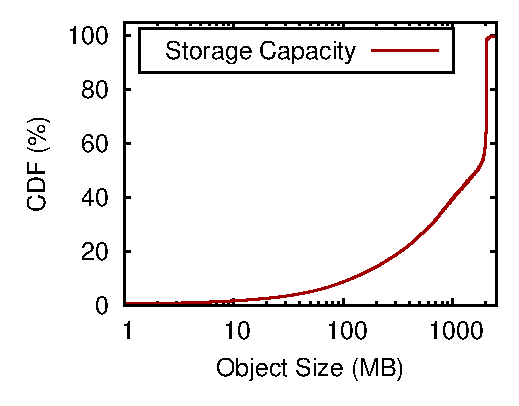
\includegraphics[width=\linewidth]{data/object_size-storage_capacity}
  \caption{}
  \label{fig:object_size-storage_capacity}
\end{subfigure}%
%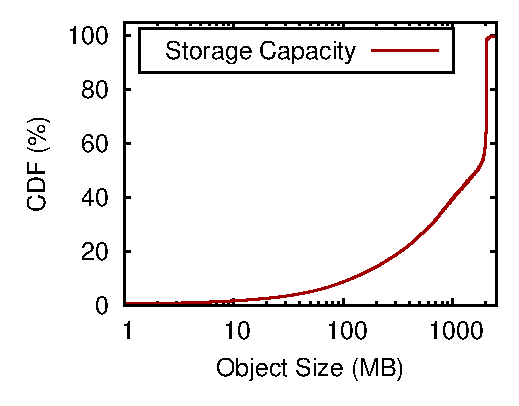
\includegraphics[width=0.5\textwidth]{data/object_size-storage_capacity}
%\hspace{-.5em}
\begin{subfigure}{.3\textwidth}
  \centering
  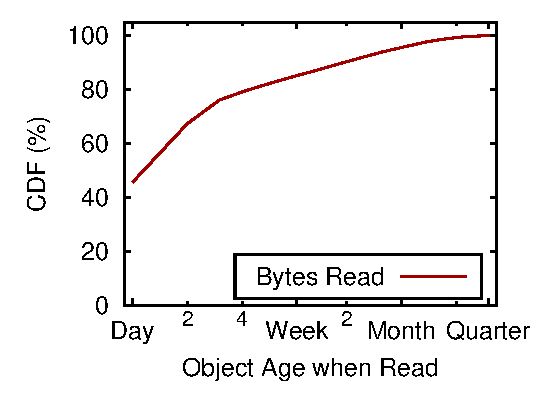
\includegraphics[width=\linewidth]{data/write_read_gap-bytes_read}
  \caption{}
  \label{fig:write_read_gap-bytes_read}
\end{subfigure}%
\caption{Cloud Drive Characteristics}
\label{fig:case_for_giza}
\end{figure}

{\bf Methodology:} The data presented in this section is derived from a three-month trace of the cloud drive service. The cloud drive serves hundreds of millions of users and stores their data objects, including documents, photos, music, videos and more. The trace includes {\em all} reads, writes and updates to {\em all} data objects between January 1 and March 31, 2016.

{\bf Large Objects Dominate:} The size of the data objects varies significantly, ranging from Kilobytes to tens of Gigabytes. While the total number of small objects vastly exceeds that of large objects, the storage capacity occupied by the small objects turns out extremely small. Indeed, Figure~\ref{fig:object_size-storage_capacity} presents the cumulative distribution of storage capacity consumption in terms of data object size. We observe that less than $0.9\%$ of the total storage capacity is occupied by data objects smaller than 4MB. This suggests that, to optimize storage cost, it is sufficient for Giza to focus on data objects of 4MB and larger~\footnote{Data objects of tens of Gigabytes are divided into 4MB chunks before storing in cloud storage back-end.}. For the same reason, data objects smaller than 4MB are filtered in the following analysis.

{\bf Object Temperature Drops Fast:} A common usage scenario of cloud drive is sharing. When data objects are stored in the cloud drive, they are often shared across multiple devices, as well as among multiple users. Therefore, it is typical to observe reads of the data objects soon after they are stored. To this end, Figure~\ref{fig:write_read_gap-bytes_read} presents the cumulative distribution of bytes read in terms of data object age when reads occur~\footnote{The analysis focuses on all the data objects created during the three-month period. Hence, the object age is capped at three months.}. It is worth pointing out that $47\%$ of the bytes read occurred in the same day as the data objects are stored, $87\%$ occurred within the same week, and merely less $2\%$ occurred beyond one month. This suggests that the temperature of the data objects stored in the cloud drive drops at a fast space. Moreover, caching the data objects for a short period of time can satisfy most of the reads (more below).

\begin{table}[h]
\centering
\begin{tabular}{|c||c|c|}
\hline \hline
total reads (B) / writes (B) 	& \multicolumn{2}{c|}{2.3$\times$}
\\ \hline \hline
%\multirow{4}{*}{cross-DC reads / writes \newline in Giza}
	& no caching		& 1.15$\times$
\\ \cline{2-3}
cross-DC reads / writes
	& caching (day)		& 0.61$\times$ 
\\ \cline{2-3}
with Giza
	& caching (week)	& 0.18$\times$ 
\\ \cline{2-3}
	& caching (month)	& 0.05$\times$ 
\\ \hline \hline
\end{tabular}
%\caption{Giza with Caching in Local DC.}
\label{tab:caching}
\end{table}
{\bf Writes Dominate with Caching:} This table further analyzes the effectiveness of caching. First of all, the ratio between the total amount of bytes due to reads and writes is 2.3$\times$. This implies that on average each data object stored in the cloud drive is read 2.3 times. As illustrated in Section~\ref{subsec:trade-off}, Giza incurs 1x and 0.5x cross-DC network traffic in writes and reads, respectively. Hence, the ratio between cross-DC network traffic due to reads and writes becomes $1.15\times$. Given the above temperature analysis, caching is most effective and it is reasonable for Giza to additionally cache entire data objects for a short period of time within one single DC. Since reads served from the DC cache incur no cross-DC network traffic, the ratio between cross-DC network traffic due to reads and writes reduces dramatically with caching. Indeed, when data objects are cached for one day, the ratio reduces to 0.61$\times$. When data objects are cached for one month, the ratio reduces to negligible 0.05$\times$, in which case, the cross-DC network traffic is completely dominated by writes.

\begin{table}[h]
\centering
\begin{tabular}{c||c|c|c}
\# of Version 	& 	1				& 2					& $\ge 3$
\\ \hline
Percentage			& $57.96\%$	& $40.88\%$	& $1.16\%$
\end{tabular}
\label{tab:version}
\end{table}
{\bf Concurrency Rare, but Versioning Required:} This table analyzes how often data objects are updated and require versioning support. We observe that $57.96\%$ of the data objects are written once and never updated during the three-month period. For the remaining, $40.88\%$ of the data objects are updated exactly once and merely $1.16\%$ are updated more than twice. This suggests that concurrent updates of data objects are rare in Giza (albeit possible). Hence, Giza focuses and optimizes for single writer, while at the same time supports versioning.

%\subsection{Giza: Flexible Cross-DC erasure coding }
%
%Erasure coding across geo-graphically distributed data centers is a most effective approach to reduce storage cost while achieving the fault tolerance goal of being able to survive data center failure. As Facebook's F4 system~\ref{bib:F4} has demonstrated, replacing geo-replication with cross-DC erasure coding can effectively reduce storage overhead from 3.6x to 2.1x, achieving huge savings for Facebook's 65PB of warm storage. While a fixed 2 + 1 solution works very well for Facebook's special workload, the public cloud storage desires much more flexibility. Different customers have different desirable operating points in terms of cost, durability and latency trade-off and are willing to accept different pricing for individual needs. 
%
%Giza provide completes flexibility to the customers. When a storage account is created, the customers may specify how much fault tolerance is desired at the storage account level. In addition, the customers had additional flexibility to specify which data centers are involved, so that they could constraint all the data to be in the  United States per data sovereignty requirement and regulation, or they could choose to disperse the erasure coded data across multiple continents, so that no single country could gain access to the complete data. 


\begin{table*}[tp]
\centering
\begin{tabular}{|l||c||c|c|c|c||c|c|}
\hline
				& Geo-Replication    	& \multicolumn{4}{c||}{Giza (standard durability)}		& \multicolumn{2}{c|}{Giza (enhanced durability)}
\\ \hline \hline
Number of DCs 				& 2										& 3 & 4 & 5 & 6									& 5 & 6
\\ \hline
Erasure coding scheme & replication					& 2 + 1 & 3 + 1 & 4 + 1 & 5 + 1	& 3 + 2 & 4 + 2
\\ \hline \hline
Storage overhead			& 2.6x								& 1.9x & 1.7x & 1.6x & 1.5x			& 2.1x & 1.9x
\\ \hline
Reduction							& -										& 27\% & 35\% & 38\% & 42\%			& 19\% & 27\%
\\ \hline \hline
WAN traffic (put)			& 1x									& 1x & 1x & 1x & 1x 						& 1.33x & 1.25x
\\ \hline
WAN traffic (get)			& 0										& 0.5x & 0.67x & 0.75x & 0.8x		& 0.67x & 0.75x
\\ \hline
DC rebuild 						& 1x									& 2x & 3x & 4x & 5x 						& 3x & 4x
\\ \hline \hline
\end{tabular}
\caption{Trade-off of storage, bandwidth and durability.}
\label{tab:cost_benefit}
\end{table*}


\subsection{Storage, Bandwidth and Durability}
\label{subsec:trade-off}

Giza offers the customers the flexibility to specify erasure coding scheme, which results in different operating points in terms of storage overhead, bandwidth cost and durability.

\subsubsection{Storage and Durability}

With standard durability, Giza applies $k+1$ erasure coding, which stores $k+1$ coded fragments in different data centers and tolerates single data center failure. With enhanced durability, Giza applies $k+2$ erasure coding, which stores coded fragments in $k+2$ data centers. This tolerates arbitrary 2 data center failures and achieves much higher durability. 

Table~\ref{tab:cost_benefit} compares the costs and benefits of Giza at various operating points to geo-replication.
To tolerate single data center failure, geo-replication requires a storage overhead of $2\times1.3$ = 2.6 (where single DC storage overhead is a constant at 1.3). With $k+1$ erasure coding, where $k$ ranges from 2 to 5, Giza reduces the storage overhead to between 1.9 and 1.5, a reduction of 27\% to 42\%. Even with enhanced durability tolerating 2 data center failures, Giza again reduces the storage overhead to between 2.1 to 1.9, a reduction of 19\% to 27\%. As summarized Table~\ref{tab:cost_benefit}, compared to geo-replication, Giza achieves comparable durability while significantly reducing storage overhead, or much higher durability while still reducing storage overhead substantially.

Nevertheless, the reduction in storage overhead comes at the additional cost of inflated cross-DC network traffic, which is examined next.

\subsubsection{Constant Cross-DC Traffic for Put}

Let's revisit the example of storing the 4MB data object. In geo-replication, in addition to being stored in a local DC, the object is replicated and stored in a remote DC. The replication incurs 1x of cross-DC traffic. Giza, with $2 + 1$ erasure coding, divides the object  and generates 3 coded fragments ($a$, $b$ and $p$) with 2MB each. It stores 1 fragment in the local DC and replicates 2 fragments to two remote DCs. The replication again incurs 1x cross-DC traffic, the same as geo-replication. In general, with $k+1$ erasure coding, the cross-DC traffic is constant for both geo-replication and cross-DC erasure coding.

The analysis readily extends to $k+2$ erasure coding. As shown in Table~\ref{tab:cost_benefit}, the cross-DC traffic is slightly higher than geo-replication, inevitable to achieve higher durability.

\subsubsection{Inflated Cross-DC Traffic for Get and Rebuild}

In geo-replication, each data center has the full copy of the data object. {\em Get} can access the local DC and incur no cross-DC traffic. In contrast, with $2+1$ erasure coding, Giza can only read half of the object from the local DC. Reading the other half from a remote DC always incurs cross-DC traffic, a $0.5$$\times$ unit for {\em get}. Generalizing the argument, Table~\ref{tab:cost_benefit} shows that the higher $k$ is (in $k+1$ erasure coding), the higher cross-DC traffic {\em get} incurs.

When a data center fails, customer data originally stored at the failed DC needs to be rebuilt at a new DC. Geo-replication simply replicates every data object and thus incurs 1x of cross-DC traffic. In contrast, Giza applies erasure decoding to reconstruct missing fragments, each incurring $k$ times cross-DC traffic for arbitrary $k+m$ erasure coding.

\subsection{Alternative Approach}
\label{sec:alternative}

%\ch{It feels better to move this subsection to a later section dedicated for discussion. We could mention Haibo's work there, or better in the related work section. If we do that, the tile of this section should probably be changed to ``costs and benefits''.}

Giza treats data objects independently. To store a data object, Giza splits the object into multiple data fragments and generates parity fragments. All the coded fragments are dispersed and stored in different data centers. To retrieve the object, Giza reads enough coded fragments from the multiple data centers and reconstructs the data object. Hence, Giza always incurs cross-DC traffic when reading object.

The decision to treat data objects independently is a deliberate choice after careful considerations of alternative approaches. One viable alternative is to first aggregate objects into logical volumes and then erasure code across different volumes. For instance, objects in data center A are aggregated into $vol_A$ and those in data center B into $vol_B$. Volumes are large, say in the order of 100GB. A parity volume $vol_P$ is generated by erasure coding $vol_A$ and $vol_B$, which is stored in yet another data center C.

This approach avoids cross-DC traffic when reading individual objects, as every object is available in its entirety in one of the DCs. However, the challenge of this approach is to handle object deletion. Whenever an object is deleted from $vol_A$ in data center A, it needs to be transmitted to data center C so as to be {\em canceled} from $vol_C$. Hence, object deletion incurs cross-DC traffic. In addition, deleting objects from the logical volumes inevitably requires additional bookkeeping and garbage collection, resulting in greatly increased engineering complexity.

%%% Local Variables:
%%% mode: latex
%%% TeX-master: "main"
%%% End:
